\documentclass{standalone}
\usepackage{tikz}
\begin{document}
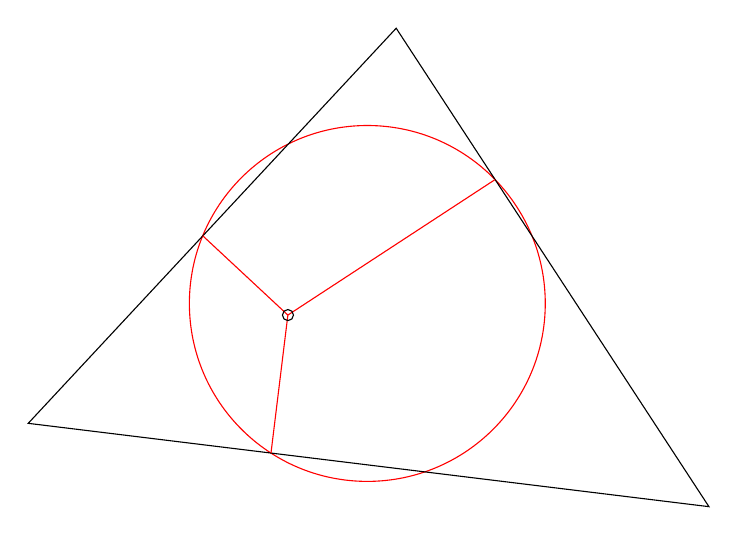
\begin{tikzpicture}[x=1pt,y=1pt]
\draw[red] (148.40,-123.95) circle (64.30);
\draw (25.87,-167.27) -- (271.84,-197.38) -- (158.83,-24.50) -- cycle;
\draw[red] (119.69,-128.15) -- (88.93,-99.50);
\draw[red] (119.69,-128.15) -- (194.57,-79.19);
\draw[red] (119.69,-128.15) -- (113.59,-178.01);
\draw (119.72,-128.15) circle (2.00);
\end{tikzpicture}
\end{document}
